\documentclass[oneside,a4paper,11pt,explicit]{article}
\usepackage[utf8]{inputenc}
\usepackage[sedes]{kultem}
\usepackage[english]{babel}
% ======================= report preamble =======================
% Loaded from main.tex after kultem.sty (kul-template skill).
% Do not edit kultem.sty itself; put additions here.

% ---------- general packages ----------
\usepackage{calc}                       % needed by \kulbox (\linewidth-2\fboxsep)
\usepackage{amsmath,amssymb,mathtools}
\usepackage{booktabs,array}
\usepackage{subcaption}
\usepackage{xcolor}
\usepackage{pgfplots}\pgfplotsset{compat=1.16}
\usepackage[accsupp]{axessibility}      % accessible PDF math (from the template)
\usepackage{upgreek}
\usepackage[hidelinks]{hyperref}

% ---------- paragraphs and lists ----------
\setlength{\parskip}{0.5em plus 0.15em minus 0.1em}
\setlist{itemsep=2pt,topsep=3pt,parsep=0pt,leftmargin=1.4em}
\captionsetup{font=small,labelfont={bf,color=Blue3}}

% ---------- section numbering like the lecture notes ----------
% \exercise{n}{Title} starts the section for problem 4.n, so skipping an
% optional problem (4.9-4.11) never shifts the numbering of the others.
\renewcommand{\thesection}{4.\arabic{section}}
\newcommand{\exercise}[2]{\setcounter{section}{\numexpr#1-1\relax}\section{#2}}

% Unnumbered section that still appears in the TOC and the footer.
\newcommand{\unnumberedsection}[1]{%
  \section*{#1}\addcontentsline{toc}{section}{#1}\markboth{#1}{}}

% Wider number column in the table of contents ("4.16" does not fit in 1.5em).
\makeatletter
\patchcmd{\l@section}{1.5em}{2.7em}{}{}
\patchcmd{\l@subsection}{2.3em}{3.2em}{}{}
\makeatother

% ---------- figures ----------
% Plots from the exercise scripts live in ../Exercises/<exercise>/figures/.
% img/ is listed too, because kultem.sty loads its logos from img/.
\graphicspath{{../Exercises/}{img/}}

% ---------- notation ----------
\newcommand{\Tc}{T_{\mathrm c}}
\newcommand{\taueq}{\tau_{\mathrm{eq}}}
\newcommand{\avg}[1]{\left\langle #1 \right\rangle}


%% TITLE PAGE
\title{Advanced Monte Carlo Simulations}
\subtitle{Report on the exercises}
\date{Academic year 2026--2027}
\author{Mathias Meersschaut \\ r0998972}
\professor{Enrico Carlon}

\begin{document}
\maketitle
\pagebreak

\tableofcontents
\pagebreak

% ---------------------------------------------------------------
\unnumberedsection{Introduction}
% Introduction: purpose of the report, programming language and tools,
% general conventions (k_B = 1, J = 1, MC sweep = one attempted update per
% spin/particle, seeds, error-bar method), and where the code can be found.


% ---------------------------------------------------------------
% One file per problem. Required: 4.1-4.8 and 4.12-4.16.
% Optional: at least one of 4.9, 4.10, 4.11 (comment out the ones you skip).
% Problem 4.1: Non-uniform random numbers
% Notes and checklist: ../Exercises/4.01-non-uniform-random-numbers/README.md
% Figures:            \includegraphics{4.01-non-uniform-random-numbers/figures/<name>}
\exercise{1}{Non-uniform random numbers}

A computer only provides uniform random numbers $u \in [0,1)$. This problem turns them into
numbers with a prescribed density $f(x)$ ($f \ge 0$, $\int f = 1$) in two ways: by inverting the
cumulative distribution function (CDF) and by the hit-and-miss (rejection) method
\cite{Carlon2025}. All runs use \texttt{numpy.random.default\_rng} with seed~1.

\subsection{Inverse CDF method}

Let $F(x) = \int_{-\infty}^{x} f(y)\,dy$. Because $f \ge 0$, $F$ is non-decreasing, and where
$f > 0$ it is strictly increasing and invertible. If $u$ is uniform on $[0,1]$ and $y = F^{-1}(u)$, then
\begin{equation}
  P(y \le t) = P\big(F^{-1}(u) \le t\big) = P\big(u \le F(t)\big) = F(t),
\end{equation}
since $P(u \le a) = a$ for $a \in [0,1]$. The CDF of $y$ is therefore $F$, and its density is
$F'(t) = f(t)$.

The three requested densities have CDFs that can be inverted by hand:
\begin{align}
  f(x) &= \tfrac13 \text{ on } [-2,1]: & F(x) &= \tfrac{x+2}{3}, & x &= -2 + 3u, \\
  f(x) &= e^{-x} \text{ on } [0,\infty): & F(x) &= 1 - e^{-x}, & x &= -\ln(1-u), \\
  f(x) &= \tfrac{x+1}{2} \text{ on } [-1,1]: & F(x) &= \tfrac{(x+1)^2}{4}, & x &= 2\sqrt{u} - 1 .
\end{align}
We use $\ln(1-u)$ instead of $\ln u$, because $u = 0$ can occur and $1-u$ is never zero.
Figure~\ref{fig:4.1-inverse} shows that the histograms of $10^5$ numbers follow the exact densities
within the Poisson error bars $\sqrt{k}$ of a bin with $k$ entries.

\begin{figure}[htbp]
  \centering
  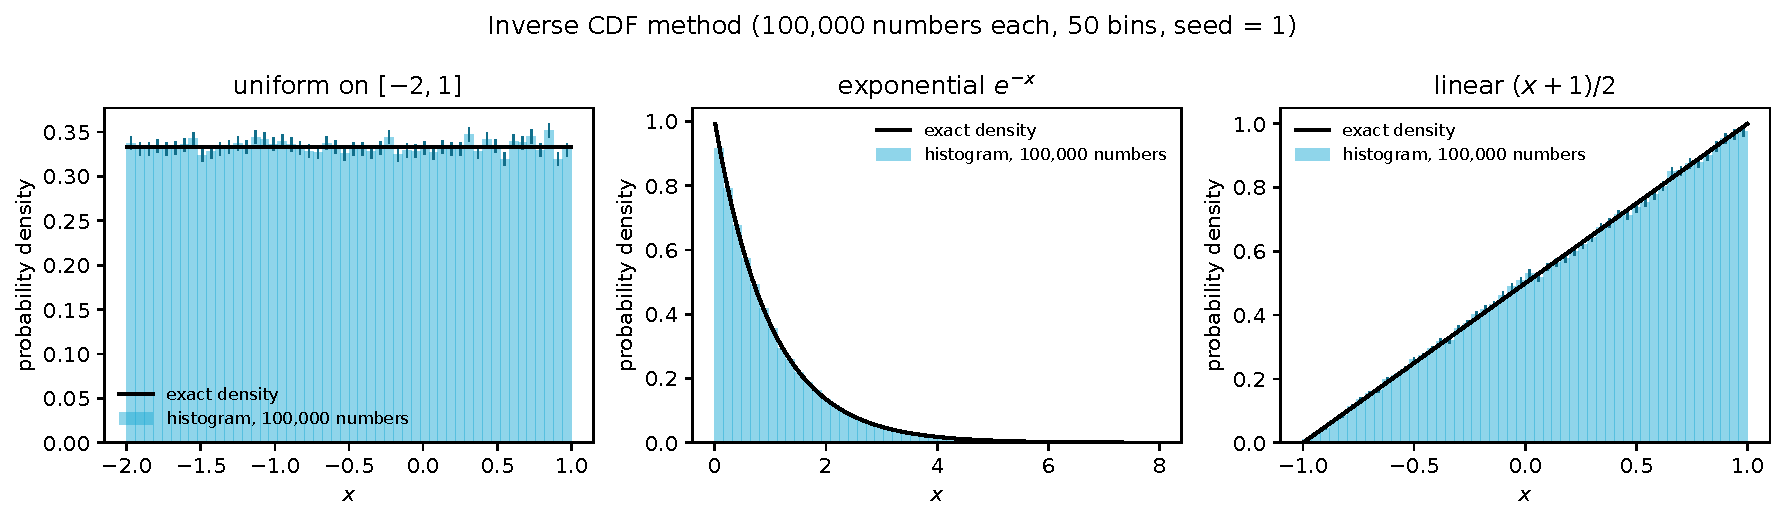
\includegraphics[width=\linewidth]{4.01-non-uniform-random-numbers/figures/a_inverse_cdf}
  \caption{Inverse CDF method: normalised histograms (50 bins, error bars $\sqrt{k}/(N\Delta x)$)
    of $N = 10^5$ numbers per density, with the exact density as a black line. Seed 1. The
    exponential histogram is cut at $x = 8$.}
  \label{fig:4.1-inverse}
\end{figure}

\subsection{Hit-and-miss method}

For $f$ supported on $[a,b]$ and bounded by $M$, we draw $t \sim U[a,b]$ and $s \sim U[0,M]$ and keep
$t$ if $s \le f(t)$. The pair $(t,s)$ is uniform in the box $[a,b]\times[0,M]$, so the kept points are
uniform in the region under the curve. The number of kept points near $t$ is proportional to the
height $f(t)$, so the kept $t$ have density $f$. This also works when $f$ is not normalised, because
only the shape of $f$ matters.

The fraction of kept points is the area under the curve divided by the area of the box,
\begin{equation}
  p_{\text{acc}} = \frac{\int_a^b f(x)\,dx}{M(b-a)} .
\end{equation}
For the linear density on $[-1,1]$ with $M = 1$ this is $1/2$. The second function,
$f(x) = -x(1-x)\,e^{-x^2}\ln(1-x)$ on $[0,1]$, is not normalised. Its maximum on a fine grid,
increased by 1\,\% to be safe, gives $M = 0.1582$, and numerical integration
(\texttt{scipy.integrate.quad}) gives $Z = \int_0^1 f = 0.09011$, so $p_{\text{acc}} = Z/M = 0.5697$.

\begin{table}[htbp]
  \centering
  \caption{Fraction of kept points in hit-and-miss, from $10^6$ tries each (seed 1). The error is
    the binomial standard error $\sqrt{p(1-p)/N_{\text{tries}}}$.}
  \label{tab:4.1-acceptance}
  \begin{tabular}{lccc}
    \toprule
    density & box & kept fraction & expected \\
    \midrule
    $(x+1)/2$ on $[-1,1]$                 & $[-1,1]\times[0,1]$      & $0.5007 \pm 0.0005$ & $0.5$ \\
    $-x(1-x)e^{-x^2}\ln(1-x)$ on $[0,1]$  & $[0,1]\times[0,0.1582]$  & $0.5705 \pm 0.0005$ & $0.5697$ \\
    unit disk (section~\ref{sec:4.1-disk}) & $[-1,1]^2$              & $0.7853 \pm 0.0004$ & $\pi/4 = 0.7854$ \\
    \bottomrule
  \end{tabular}
\end{table}

The measured fractions in table~\ref{tab:4.1-acceptance} agree with the prediction within 1.6
standard errors, and the histograms in figure~\ref{fig:4.1-hm} follow the (normalised) densities.
The method wastes the rejected points, so a box that fits $f$ tightly (small $M$) is more efficient.
A larger $M$ gives the same distribution, only at a lower acceptance rate.

\begin{figure}[htbp]
  \centering
  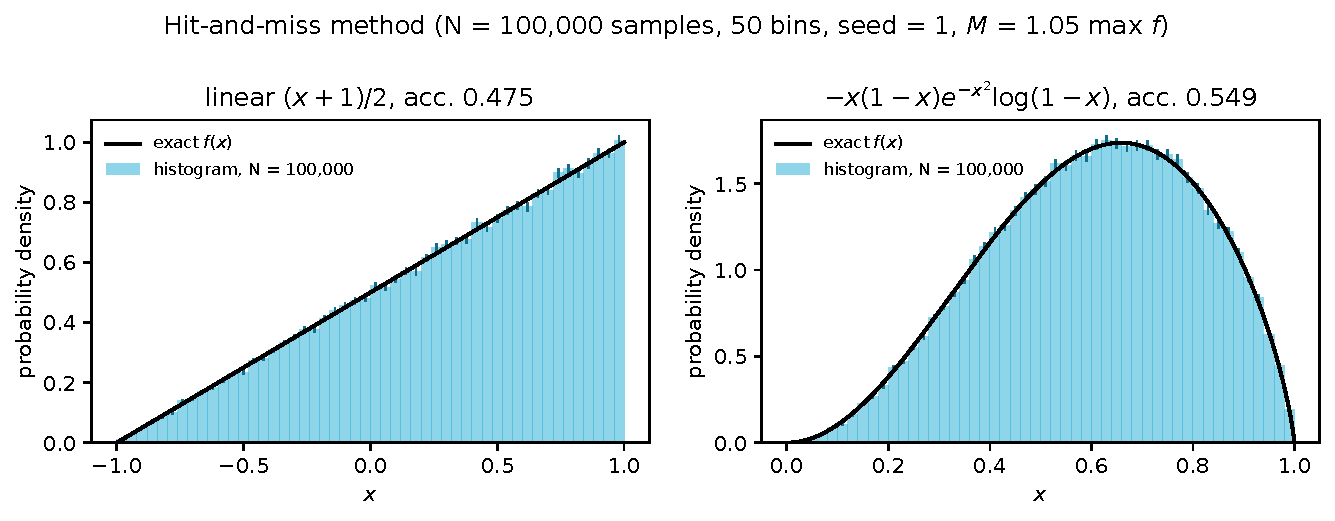
\includegraphics[width=0.9\linewidth]{4.01-non-uniform-random-numbers/figures/b_hit_and_miss}
  \caption{Hit-and-miss method with $10^6$ tries per density: histograms (50 bins) of the
    $500\,745$ and $570\,481$ kept numbers. The second density is divided by $Z = 0.09011$ to
    compare with the normalised histogram. Box heights $M = 1$ and $M = 0.1582$, seed 1.}
  \label{fig:4.1-hm}
\end{figure}

\subsection{Uniform points in a disk with hit-and-miss}
\label{sec:4.1-disk}

Points $(x,y)$ uniform in the square $[-1,1]^2$ are kept when $x^2 + y^2 \le 1$. The kept points are
uniform in the unit disk (figure~\ref{fig:4.1-disk}, left). The kept fraction is the area ratio
$\pi/4$, which gives a Monte Carlo estimate of $\pi$ as a by-product:
\begin{equation}
  \pi \approx 4 \times 0.7853 = 3.1410 \pm 0.0016 .
\end{equation}

\subsection{Uniform points in a disk in polar coordinates}

A uniform density on the unit disk is $1/\pi$ per unit area. With the area element
$dA = r\,dr\,d\theta$ this becomes
\begin{equation}
  f(r,\theta)\,dr\,d\theta = \frac{1}{\pi}\, r\,dr\,d\theta
  = \underbrace{2r\,dr}_{r \in [0,1]} \; \underbrace{\frac{d\theta}{2\pi}}_{\theta \in [0,2\pi)} .
\end{equation}
The density factorises, so $r$ and $\theta$ are independent. The angle is uniform,
$\theta = 2\pi v$, and the radius has $F(r) = r^2$, so the inverse CDF method of the first subsection gives
$r = \sqrt{u}$, with $u$ and $v$ two independent uniform numbers. No point is rejected.

\kulbox[5pt]{Uniform points in the unit disk without rejection: $\theta = 2\pi v$ and $r = \sqrt{u}$.
The square root comes from the Jacobian $r$ of the polar coordinates.}

The naive choice $r = u$ gives a flat radial density instead of $2r$: the same number of points
lands in every ring, while the area of a ring grows with $r$. The points then pile up near the centre
(figure~\ref{fig:4.1-disk}, right). Figure~\ref{fig:4.1-radial} confirms that both correct methods give
the radial density $2r$, and that $r = u$ does not.

\begin{figure}[htbp]
  \centering
  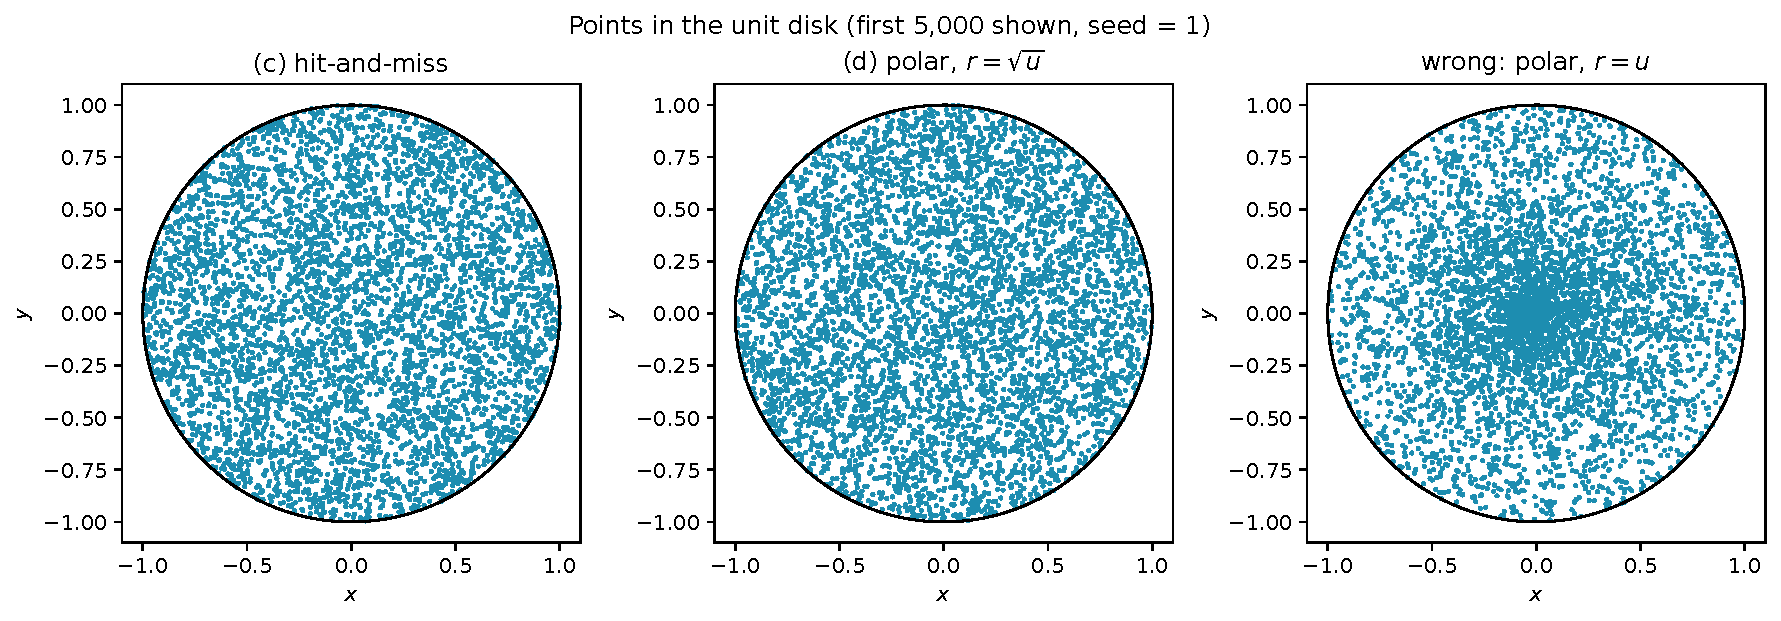
\includegraphics[width=\linewidth]{4.01-non-uniform-random-numbers/figures/cd_disk_scatter}
  \caption{Points in the unit disk (the first 5\,000 shown). Left: hit-and-miss in $[-1,1]^2$,
    $10^6$ tries. Middle: polar coordinates with $r = \sqrt{u}$, $N = 10^5$. Right: the wrong choice
    $r = u$, $N = 10^5$, which crowds the centre. Seed 1.}
  \label{fig:4.1-disk}
\end{figure}

\begin{figure}[htbp]
  \centering
  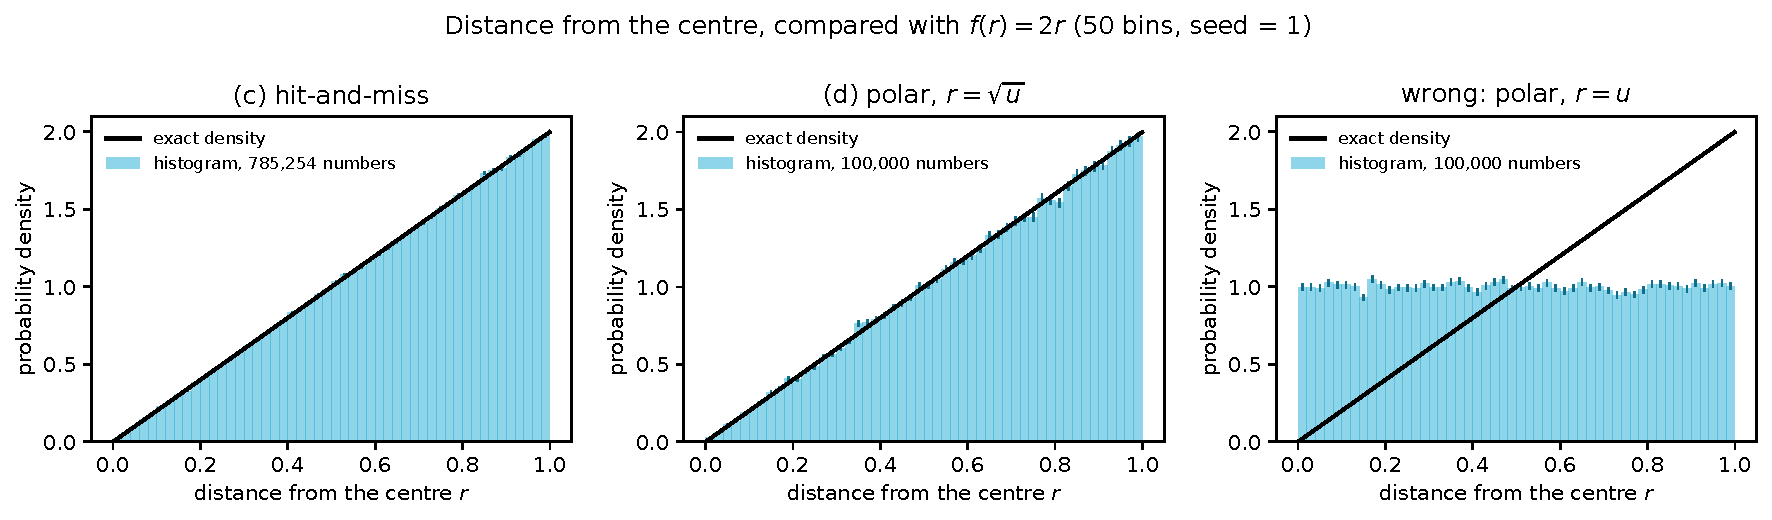
\includegraphics[width=\linewidth]{4.01-non-uniform-random-numbers/figures/cd_radial_density}
  \caption{Histograms (50 bins) of the distance $r$ to the centre for the three samples of
    figure~\ref{fig:4.1-disk} ($785\,254$ kept hit-and-miss points, $10^5$ polar points each),
    compared with the density $f(r) = 2r$ of a uniform disk. Seed 1.}
  \label{fig:4.1-radial}
\end{figure}

% Problem 4.2: Gaussian RNG
% Notes and checklist: ../Exercises/4.02-gaussian-rng/README.md
% Figures:            \includegraphics{4.02-gaussian-rng/figures/<name>}
\exercise{2}{Gaussian RNG}

The CDF of a single Gaussian is the error function, which has no closed-form inverse, so the
method of problem~4.1 does not apply directly. The Box--Muller method avoids this by generating
two Gaussian numbers at once, in polar coordinates \cite{Carlon2025}.

\subsection{The Box--Muller algorithm}

Two independent standard normal numbers $x, y$ have the joint density
$\frac{1}{2\pi} e^{-(x^2+y^2)/2}\,dx\,dy$. In polar coordinates, with $dx\,dy = r\,dr\,d\theta$,
\begin{equation}
  f(r,\theta)\,dr\,d\theta
  = \underbrace{r\,e^{-r^2/2}\,dr}_{r \in [0,\infty)} \; \underbrace{\frac{d\theta}{2\pi}}_{\theta \in [0,2\pi)} .
\end{equation}
The factor $r$ from the Jacobian makes the radial density integrable in closed form:
\begin{equation}
  F(r) = \int_0^r e^{-z^2/2} z\,dz = 1 - e^{-r^2/2}
  \quad\Longrightarrow\quad
  r = \sqrt{-2\ln(1-u_1)}, \qquad \theta = 2\pi u_2 ,
\end{equation}
after which $x = r\cos\theta$ and $y = r\sin\theta$. Because the density factorises in $r$ and
$\theta$, the two must be drawn from two \emph{independent} uniform numbers $u_1, u_2$. Using the same
$u$ for both makes $r$ a function of $\theta$, and all points lie on one spiral; this was a bug
in a first version of the code.

The density also factorises in Cartesian coordinates, $\frac{1}{2\pi}e^{-(x^2+y^2)/2} = \phi(x)\,\phi(y)$
with $\phi$ the standard normal density. So $x$ and $y$ are not only normal but independent.

\begin{figure}[htbp]
  \centering
  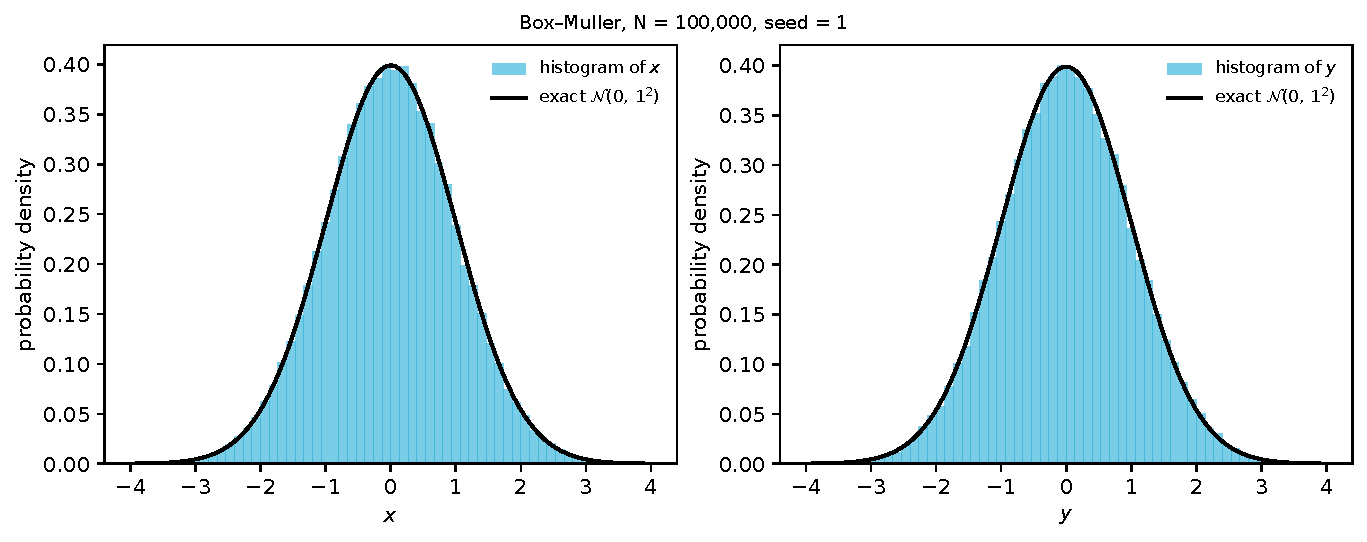
\includegraphics[width=0.9\linewidth]{4.02-gaussian-rng/figures/box_muller_hist}
  \caption{Box--Muller: histograms (60 bins) of $x$ and $y$ from $N = 10^5$ pairs, with the exact
    $\mathcal N(0,1)$ density. Seed 1.}
  \label{fig:4.2-hist}
\end{figure}

\begin{table}[htbp]
  \centering
  \caption{Sample moments of $N = 10^5$ Box--Muller pairs (seed 1). The error on the mean is
    $s/\sqrt N$. For (b) the same pairs are rescaled.}
  \label{tab:4.2-moments}
  \begin{tabular}{llcc}
    \toprule
    case & variable & mean & variance \\
    \midrule
    (a) $\mathcal N(0,1)$             & $x$  & $-0.0033 \pm 0.0032$ & $0.995$ \\
                                      & $y$  & $+0.0072 \pm 0.0032$ & $1.004$ \\
    (b) $\mu = 3$, $\sigma = 2$       & $x'$ & $2.9934 \pm 0.0063$  & $3.981$ \\
                                      & $y'$ & $3.0145 \pm 0.0063$  & $4.014$ \\
    (b) $\boldsymbol\mu = (3,-5)$, $\boldsymbol\sigma = (2,1)$
                                      & $x'$ & $2.9934 \pm 0.0063$  & $3.981$ \\
                                      & $y'$ & $-4.9928 \pm 0.0032$ & $1.004$ \\
    \bottomrule
  \end{tabular}
\end{table}

Figure~\ref{fig:4.2-hist} shows that both coordinates follow the standard normal density, and
table~\ref{tab:4.2-moments} gives means compatible with 0 and variances compatible with 1 (the
relative error on a variance from $10^5$ points is $\sqrt{2/N} \approx 0.45\,\%$). The mean of $y$ is
2.2 standard errors from zero, which is an ordinary fluctuation for one seed. The scatter plot of
figure~\ref{fig:4.2-xy} (left) is a circularly symmetric cloud, and the correlation coefficient
$\rho_{xy} = -0.0016$ is compatible with $0 \pm 1/\sqrt N = 0 \pm 0.0032$. A zero correlation alone
does not prove independence; the factorisation of the density above does.

\subsection{Mean $\mu$ and variance $\sigma^2$}

The algorithm does not need to change: the output is rescaled,
\begin{equation}
  x' = \mu + \sigma x, \qquad y' = \mu + \sigma y .
\end{equation}
Then $\avg{x'} = \mu$ and $\mathrm{Var}(x') = \sigma^2\,\mathrm{Var}(x) = \sigma^2$. The density stays
Gaussian, because the change of variables $x = (x'-\mu)/\sigma$, $dx = dx'/\sigma$ gives
$\frac{1}{\sqrt{2\pi\sigma^2}} e^{-(x'-\mu)^2/2\sigma^2}$. Equivalently, one can draw
$r = \sigma\sqrt{-2\ln(1-u_1)}$ and shift the result by $\mu$.

\kulbox[5pt]{Box--Muller: $r = \sqrt{-2\ln(1-u_1)}$, $\theta = 2\pi u_2$, then
$x = \mu + \sigma r\cos\theta$ and $y = \mu + \sigma r\sin\theta$ are two independent
$\mathcal N(\mu,\sigma^2)$ numbers.}

We tested this with $\mu = 3$, $\sigma = 2$ for both coordinates, and with different parameters per
axis, $\boldsymbol\mu = (3,-5)$ and $\boldsymbol\sigma = (2,1)$. The moments in
table~\ref{tab:4.2-moments} agree with the targets. They are the same Box--Muller pairs as in (a), so the
relative deviations are those of (a). With different $\sigma$ per axis the cloud becomes an ellipse
elongated along $x$ (figure~\ref{fig:4.2-xy}, right).

\begin{figure}[htbp]
  \centering
  \begin{subfigure}{0.46\linewidth}
    \centering
    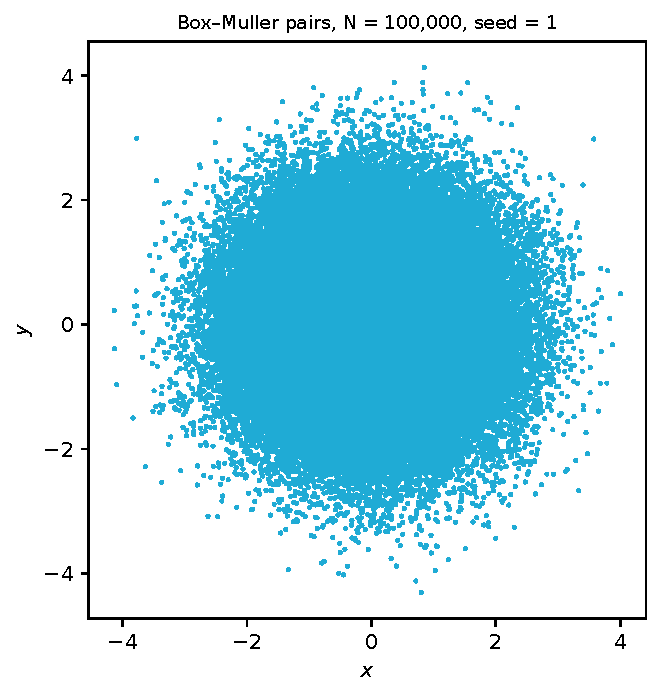
\includegraphics[width=\linewidth]{4.02-gaussian-rng/figures/box_muller_xy}
    \caption{$\mathcal N(0,1)$ for both coordinates.}
  \end{subfigure}\hfill
  \begin{subfigure}{0.46\linewidth}
    \centering
    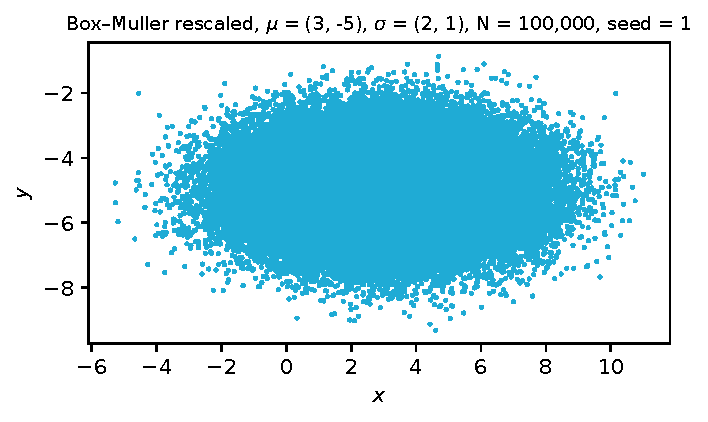
\includegraphics[width=\linewidth]{4.02-gaussian-rng/figures/box_muller_xy_mu_sigma_asym}
    \caption{$\boldsymbol\mu = (3,-5)$, $\boldsymbol\sigma = (2,1)$.}
  \end{subfigure}
  \caption{Scatter plots of $N = 10^5$ Box--Muller pairs $(x,y)$, seed 1. The rescaled pairs on the
    right are the same as on the left, shifted by $\boldsymbol\mu$ and stretched by $\boldsymbol\sigma$.}
  \label{fig:4.2-xy}
\end{figure}

% Problem 4.3: Monte Carlo integration (I)
% Notes and checklist: ../Exercises/4.03-mc-integration-1/README.md
% Figures:            \includegraphics{4.03-mc-integration-1/figures/<name>}
\exercise{3}{Monte Carlo integration (I)}

The integral to estimate is
\begin{equation}
  \mathcal I = \int_{\mathbb R^3} e^{-r^2/2}\,(x+y+z)^2\,dx\,dy\,dz, \qquad r^2 = x^2+y^2+z^2 .
\end{equation}
The Gaussian factor serves as the sampling density (importance sampling) and $(x+y+z)^2$ as the
function to average \cite{Carlon2025}. All runs use seed~1; the Gaussian numbers come from
\texttt{scipy.stats.norm.rvs}.

\subsection{Analytical value}

Expanding $(x+y+z)^2 = x^2+y^2+z^2 + 2(xy+yz+zx)$, every cross term is odd in at least one
coordinate and integrates to zero against the even Gaussian. Each square term gives
$\int x^2 e^{-x^2/2}dx \cdot \big(\int e^{-y^2/2}dy\big)^2 = \sqrt{2\pi}\cdot 2\pi = (2\pi)^{3/2}$, so
\begin{equation}
  \mathcal I = 3\,(2\pi)^{3/2} = 6\sqrt2\,\pi^{3/2} = 47.249 .
\end{equation}
A symbolic integration with \texttt{sympy} gives the same result.

\subsection{Estimate with Gaussian random numbers}

The Gaussian factor is not normalised: $e^{-r^2/2} = (2\pi)^{3/2}\,w(\mathbf r)$, where
$w(\mathbf r) = (2\pi)^{-3/2}e^{-r^2/2}$ is the density of three independent $\mathcal N(0,1)$ numbers.
Hence
\begin{equation}
  \mathcal I = (2\pi)^{3/2}\,\avg{f}_w \approx \mathcal I_N = \frac{(2\pi)^{3/2}}{N}\sum_{i=1}^{N} f(\mathbf r_i),
  \qquad f = (x+y+z)^2 ,
\end{equation}
with $\mathbf r_i$ drawn from $w$. The points are independent, so the standard error is
$(2\pi)^{3/2}s_f/\sqrt N$, with $s_f$ the sample standard deviation of the $f(\mathbf r_i)$.

\kulbox[5pt]{With $N = 10^6$ Gaussian points: $\mathcal I_N = 47.241 \pm 0.067$, compared with the
exact $\mathcal I = 47.249$, a deviation of $-0.12$ standard errors.}

\subsection{Variance of the estimate}

The central limit theorem predicts $\sigma^2(\mathcal I_N) = (2\pi)^3\,\mathrm{Var}_w(f)/N$. Here
$s = x+y+z \sim \mathcal N(0,3)$, so $s^2/3$ follows a $\chi^2_1$ distribution with variance 2, and
$\mathrm{Var}(f) = \mathrm{Var}(s^2) = 9 \cdot 2 = 18$. This gives
$\sigma^2(\mathcal I_N) = 18\,(2\pi)^3/N = 4465/N$.

To measure the variance we repeat the whole estimate $M = 1000$ times with independent points, for
13 values of $N$ from 10 to $10^5$, and take the sample variance of the 1000 values $\mathcal I_N$.
That variance is itself uncertain, with relative error $\sqrt{2/(M-1)} = 4.5\,\%$. A weighted fit of
$\ln\sigma^2$ against $\ln N$ (figure~\ref{fig:4.3-variance}) gives
\begin{equation}
  \sigma^2(\mathcal I_N) = 4441\,N^{-1.000 \pm 0.004},
\end{equation}
in agreement with the predicted exponent $-1$ and prefactor 4465. The product $N\sigma^2$ lies
between 4067 and 4750 for all $N$, each value with an error of about 200.

The spread of the individual values $f(\mathbf r_i)$ does not decrease with $N$; only the spread of
their mean does. The error $\sigma_f/\sqrt N$ is independent of the dimension of the integral: the
problem only enters through the prefactor $\sigma_f$, which depends on the chosen density.

\begin{figure}[htbp]
  \centering
  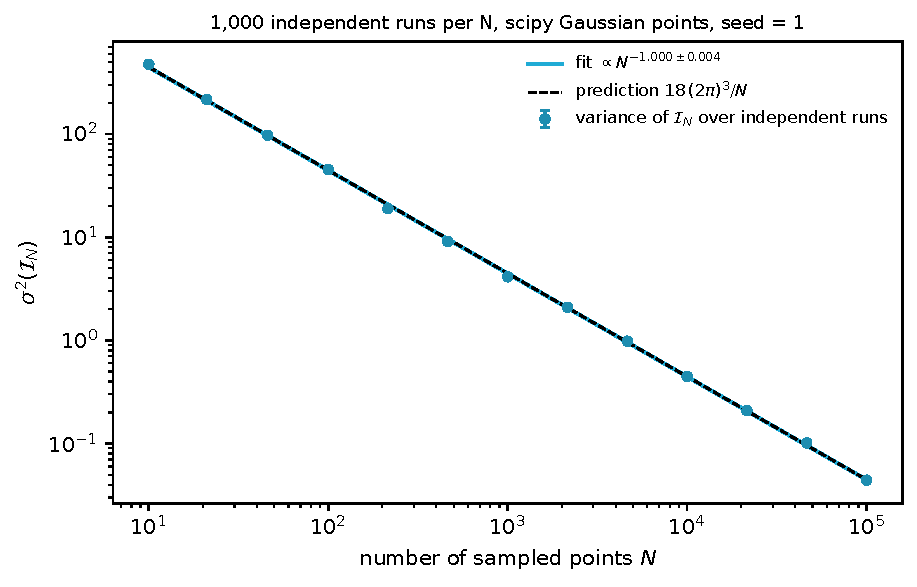
\includegraphics[width=0.75\linewidth]{4.03-mc-integration-1/figures/mc_variance}
  \caption{Variance of the importance-sampling estimate $\mathcal I_N$ over $M = 1000$ independent
    runs per $N$, for 13 log-spaced $N$ from 10 to $10^5$. Error bars $\sigma^2\sqrt{2/(M-1)}$. Line:
    weighted power-law fit; dashed: prediction $18\,(2\pi)^3/N$. Seed 1.}
  \label{fig:4.3-variance}
\end{figure}

\subsection{Why the two factors cannot be swapped}

Using $(x+y+z)^2$ as the density and $e^{-r^2/2}$ as the function to average fails for a basic
reason: a probability density must be non-negative \emph{and} normalisable. The first condition
holds, but $\int_{\mathbb R^3}(x+y+z)^2\,d^3r = \infty$, so there is no density proportional to
$(x+y+z)^2$ on $\mathbb R^3$.

To see what goes wrong in practice we restrict the integral to a box $[-L,L]^3$. There
$Z = \int_{\text{box}}(x+y+z)^2\,d^3r = (2L)^3L^2 \propto L^5$ is finite, $p = (x+y+z)^2/Z$ is a
density, and $\mathcal I_{\text{box}} = \avg{g}_p$ with $g = Z e^{-r^2/2}$. We sample $p$ by
hit-and-miss (uniform proposal in the box, acceptance $(x+y+z)^2/(3L)^2$), with $10^6$ points per box.

\begin{table}[htbp]
  \centering
  \caption{Swapped roles on the box $[-L,L]^3$: estimate of the box integral and the relative spread
    of $g$ per point, $10^6$ points per $L$ (seed 1). For comparison, the Gaussian density on
    $\mathbb R^3$ has $\sigma_f/\avg f = \sqrt{18}/3 = 1.41$ and gives $\mathcal I = 47.249$.}
  \label{tab:4.3-swapped}
  \begin{tabular}{rccccccccc}
    \toprule
    $L$ & 1 & 1.5 & 2 & 3 & 4 & 6 & 8 & 12 & 16 \\
    \midrule
    $\mathcal I_{\text{box}}$ & 4.376 & 16.94 & 31.79 & 45.68 & 47.47 & 47.15 & 46.4 & 42.4 & 44.8 \\
    error                     & 0.001 & 0.01  & 0.03  & 0.12  & 0.26  & 0.72  & 1.4  & 3.5  & 7.4 \\
    $\sigma_g/\avg g$         & 0.24  & 0.55  & 1.00  & 2.61  & 5.44  & 15.4  & 30.2 & 81.4 & 166 \\
    \bottomrule
  \end{tabular}
\end{table}

Table~\ref{tab:4.3-swapped} and figure~\ref{fig:4.3-swapped} show the dilemma. A small box is precise
but biased, because it cuts off part of the Gaussian. A large box contains the whole Gaussian but is
noisy: the relative spread per point grows as $L^{5/2}$ (doubling $L$ multiplies it by about
$2^{5/2} = 5.7$), and the limit $L \to \infty$ does not exist. The cause is that the density
$\propto (x+y+z)^2$ puts most points at large $|x+y+z|$, where the integrand $e^{-r^2/2}$ is
practically zero. A good importance-sampling density follows the shape of the integrand, so the
ratio integrand/density is nearly constant; $e^{-r^2/2}$ does this, $(x+y+z)^2$ does the opposite.

\begin{figure}[htbp]
  \centering
  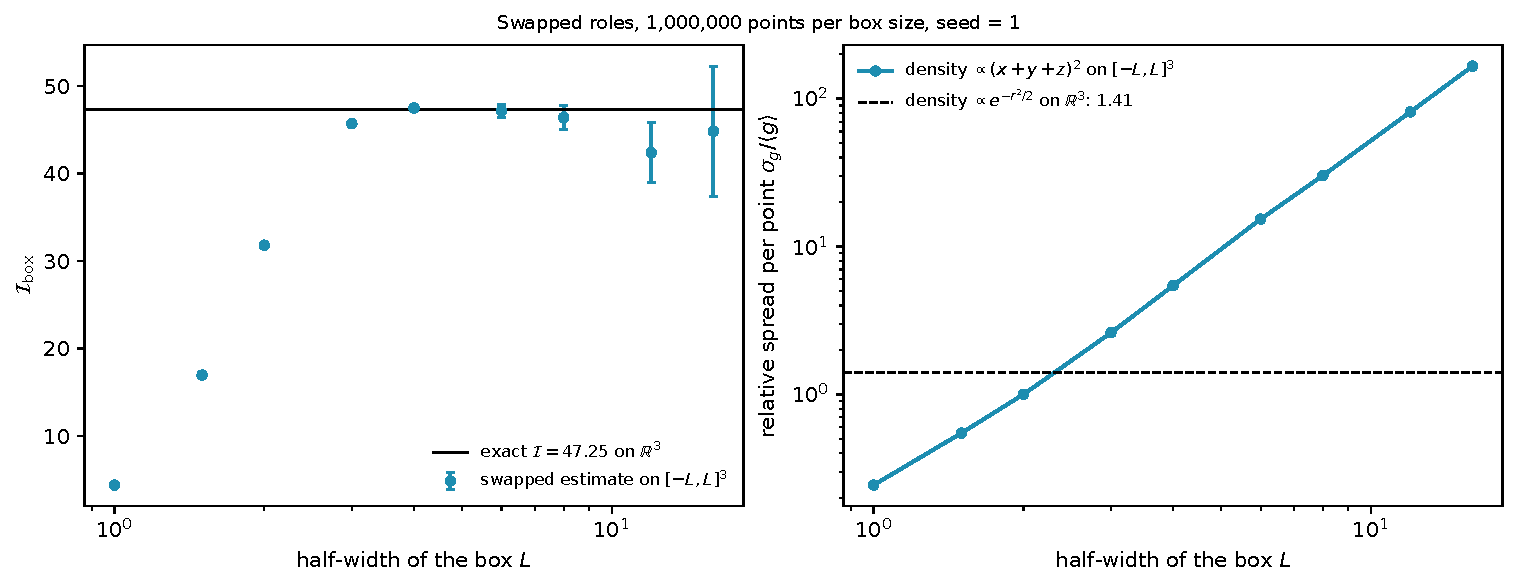
\includegraphics[width=\linewidth]{4.03-mc-integration-1/figures/mc_swapped}
  \caption{Swapped roles, density $\propto(x+y+z)^2$ on $[-L,L]^3$, $10^6$ points per box size
    (seed 1). Left: estimate of the box integral against $L$, with the exact $\mathcal I$ on
    $\mathbb R^3$. Right: relative spread per point $\sigma_g/\avg g$, compared with the Gaussian
    density (dashed).}
  \label{fig:4.3-swapped}
\end{figure}

% Problem 4.4: Monte Carlo integration (II)
% Notes and checklist: ../Exercises/4.04-mc-integration-2-metropolis/README.md
% Figures:            \includegraphics{4.04-mc-integration-2-metropolis/figures/<name>}
\exercise{4}{Monte Carlo integration (II)}

The integral $\mathcal I$ of problem~4.3 is now computed with points from a Markov chain whose
stationary distribution is $w(\mathbf r) = (2\pi)^{-3/2}e^{-r^2/2}$, built with the Metropolis
algorithm \cite{Carlon2025}. One step from the current point $\mathbf r$:
\begin{enumerate}
  \item propose $\mathbf r' = \mathbf r + \boldsymbol\delta$, with the three components of
        $\boldsymbol\delta$ independent and uniform in $[-h/2, h/2]$;
  \item accept with probability $A = \min\big(1, e^{-(r'^2-r^2)/2}\big)$, otherwise keep $\mathbf r$.
        A rejected move still counts: the old point is added to the sample again.
\end{enumerate}
The proposal is symmetric, $g(\mathbf r\to\mathbf r') = g(\mathbf r'\to\mathbf r)$, so
$P(\mathbf r\to\mathbf r')/P(\mathbf r'\to\mathbf r) = A(\mathbf r\to\mathbf r')/A(\mathbf r'\to\mathbf r)
= w(\mathbf r')/w(\mathbf r)$, which is detailed balance. Every point can be reached in a finite
number of steps for any $h > 0$, so the chain is ergodic and $w$ is its unique stationary
distribution. Only the ratio $w(\mathbf r')/w(\mathbf r)$ enters, so the normalisation of $w$ is not
needed. All runs use seed~1 with one generator used in order through the notebook.

\subsection{Trajectories and equilibrium distribution}

Figure~\ref{fig:4.4-traj} shows the $(x,y)$ projection of chains of $10^4$ steps. With $h = 1$
(acceptance 0.81) the chain from the origin fills the Gaussian blob $|x|,|y| \lesssim 3$, and the chain
from $(10,10,10)$ walks to the origin in a few hundred steps and then stays there. With $h = 0.1$
(acceptance 0.94--0.99) the chain performs a slow random walk: from the origin it explores only a part
of the blob, and from $(10,10,10)$ it only just reaches the centre at the end of the run.

\begin{figure}[htbp]
  \centering
  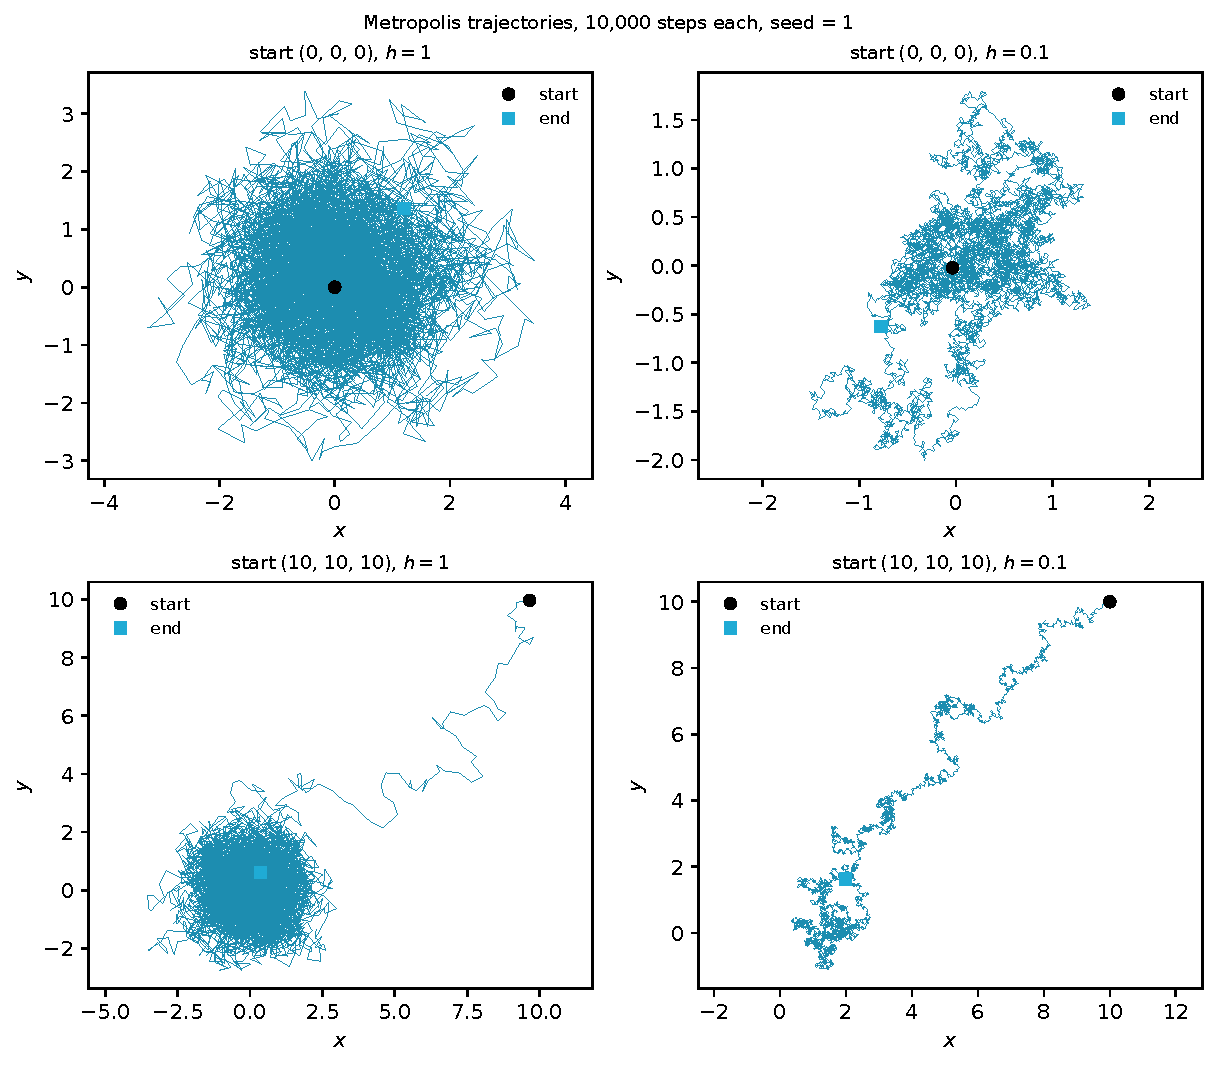
\includegraphics[width=0.72\linewidth]{4.04-mc-integration-2-metropolis/figures/trajectories}
  \caption{$(x,y)$ projection of Metropolis chains of $10^4$ steps, starting at $(0,0,0)$ (top) and
    $(10,10,10)$ (bottom), with step size $h = 1$ (left) and $h = 0.1$ (right). Acceptance rates 0.81,
    0.99, 0.81 and 0.94. Seed 1.}
  \label{fig:4.4-traj}
\end{figure}

To check the stationary distribution we run $10^6$ steps from the origin, after discarding $2\times10^4$
equilibration steps (well above the $N_{\text{eq}}$ found in the third subsection). The histograms in
figure~\ref{fig:4.4-hist} follow the exact marginals, $e^{-x^2/2}/\sqrt{2\pi}$ for each coordinate and
the Maxwell density $\sqrt{2/\pi}\,r^2e^{-r^2/2}$ for $r = |\mathbf r|$. For $h = 1$ the second moments
are $\avg{x^2}, \avg{y^2}, \avg{z^2} = 1.002, 1.000, 1.001$ (exact 1). For $h = 0.1$ they are $1.023,
0.964, 1.025$ and the histograms are visibly noisier: the same number of points, but far fewer
independent ones.

\begin{figure}[htbp]
  \centering
  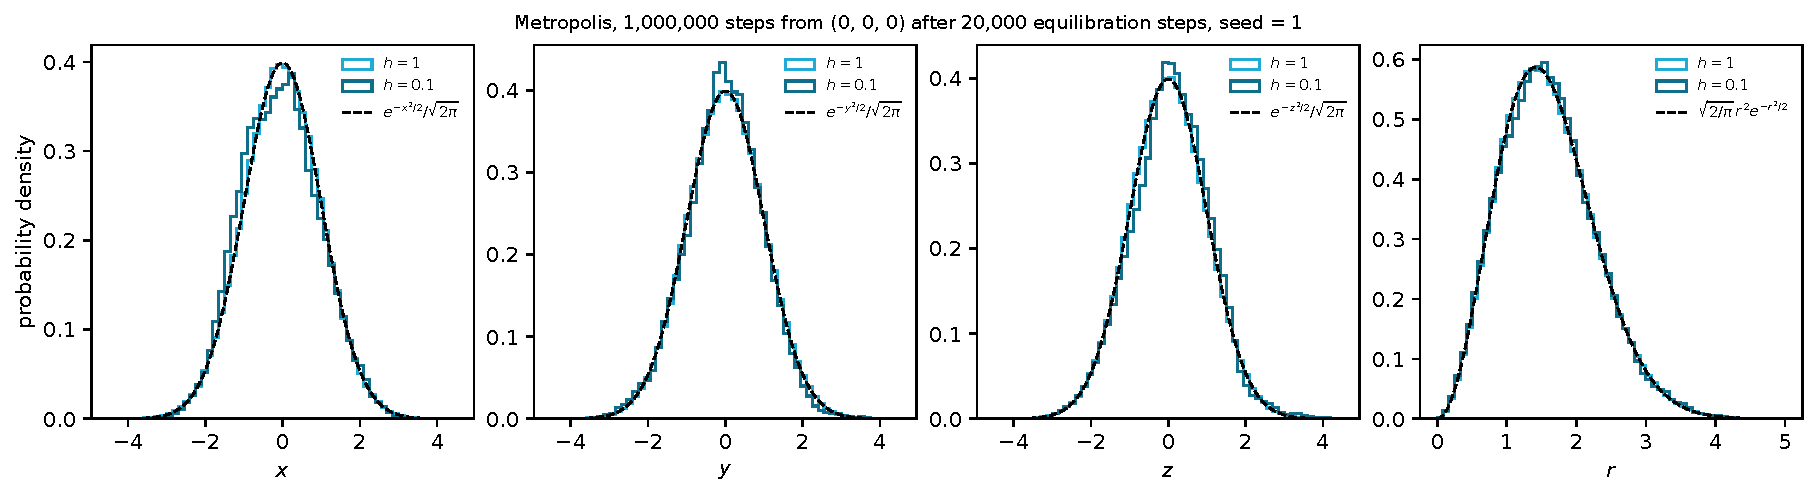
\includegraphics[width=\linewidth]{4.04-mc-integration-2-metropolis/figures/histograms}
  \caption{Histograms (60 bins) of $x$, $y$, $z$ and $r$ from Metropolis chains of $10^6$ steps
    started at the origin, after $2\times10^4$ discarded equilibration steps, for $h = 1$ and
    $h = 0.1$. Dashed: exact densities. Seed 1.}
  \label{fig:4.4-hist}
\end{figure}

\subsection{Estimate of the integral}

As in problem~4.3, $\mathcal I = (2\pi)^{3/2}\avg{f}_w$ with $f = (x+y+z)^2$, but the average now runs
over the points of the chain. Successive points are correlated, so the naive error $s_f/\sqrt N$ is too
small. We use blocking: the chain is cut into blocks of $B$ steps, and the spread of the block means
gives the error. When $B$ is much longer than the correlation time the block means are independent,
and the error stops growing with $B$ (figure~\ref{fig:4.4-blocking}). The error at $B = 8192$ defines
the integrated autocorrelation time through
$\sigma_{\text{block}}^2 = 2\tau_{\text{int}}\,s_f^2/N$.

\begin{table}[htbp]
  \centering
  \caption{Estimates of $\mathcal I$ with $N = 10^6$ points. Metropolis: chains from the origin after
    $2\times10^4$ discarded steps, error from blocking with $B = 8192$. Seed 1.}
  \label{tab:4.4-integral}
  \begin{tabular}{lcccc}
    \toprule
    method & $\mathcal I$ & naive error & $\tau_{\text{int}}$ (steps) & deviation \\
    \midrule
    exact                       & $47.249$           & --    & --          & -- \\
    Gaussian sampling (4.3)     & $47.241 \pm 0.067$ & 0.067 & $1/2$       & $-0.1\sigma$ \\
    Metropolis, $h = 1$         & $47.64 \pm 0.42$   & 0.067 & $19 \pm 2$   & $+0.9\sigma$ \\
    Metropolis, $h = 0.1$       & $43.5 \pm 2.3$     & 0.059 & $770 \pm 100$ & $-1.6\sigma$ \\
    \bottomrule
  \end{tabular}
\end{table}

\kulbox[5pt]{Metropolis with $N = 10^6$ steps gives $\mathcal I = 47.64 \pm 0.42$ ($h = 1$) and
$43.5 \pm 2.3$ ($h = 0.1$), both compatible with the exact $47.249$. The error is $\sqrt{2\tau_{\text{int}}}$
times that of direct Gaussian sampling: 6 times larger for $h = 1$ and 40 times for $h = 0.1$.}

The naive errors in table~\ref{tab:4.4-integral} are about the same as for Gaussian sampling, because
the points have the right distribution. They ignore the correlations and are therefore wrong. For
$h = 0.1$ the blocking curve has not fully levelled off at $B = 8192$ (the chain contains only about
$N/2\tau_{\text{int}} \approx 600$ independent points), so that error bar is a slight underestimate.

\begin{figure}[htbp]
  \centering
  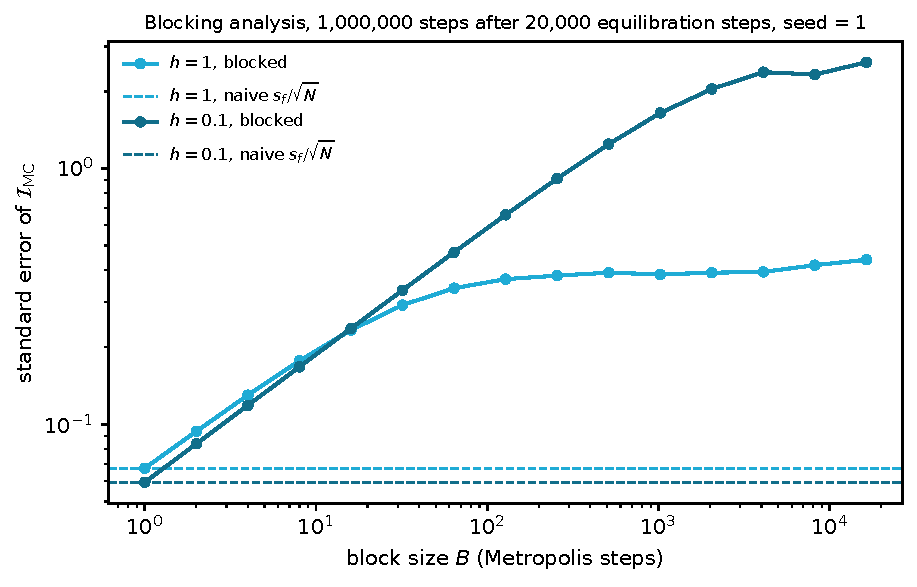
\includegraphics[width=0.72\linewidth]{4.04-mc-integration-2-metropolis/figures/blocking}
  \caption{Blocking analysis: standard error of $\mathcal I_{\text{MC}}$ against block size $B$ for the
    $10^6$-step chains of figure~\ref{fig:4.4-hist}. Dashed: the naive error $s_f/\sqrt N$ ($B = 1$).
    Seed 1.}
  \label{fig:4.4-blocking}
\end{figure}

\subsection{Equilibration time}

Starting from $(10,10,10)$, $r^2 = 300$ has to relax to its equilibrium mean $\avg{r^2} = 3$. One chain is
noisy, so we average $r^2(t)$ over 100 independent chains of $2\times10^4$ steps. In equilibrium
$r^2 \sim \chi^2_3$ has variance 6, so the chain average fluctuates by $\sqrt{6/100} = 0.24$. We define
$N_{\text{eq}}$ as the first step at which the average drops below $3 + 2\sqrt{6/100} = 3.49$
(figure~\ref{fig:4.4-eq}).

For small $h$ the relaxation can be estimated. A uniform step has variance $h^2/12$ per component, and to
first order Metropolis gives a mean displacement $\frac{h^2}{24}\nabla\ln w = -\frac{h^2}{24}\mathbf r$
per step. Then $\avg{r^2} - 3 \approx 297\,e^{-h^2t/12}$, so
\begin{equation}
  N_{\text{eq}} \approx \frac{12}{h^2}\ln\frac{297}{0.49} \propto \frac{1}{h^2} .
\end{equation}

\begin{table}[htbp]
  \centering
  \caption{Equilibration time from $(10,10,10)$, 100 chains of $2\times10^4$ steps, seed 1.}
  \label{tab:4.4-neq}
  \begin{tabular}{ccc}
    \toprule
    $h$ & measured $N_{\text{eq}}$ & small-$h$ estimate \\
    \midrule
    1   & 205  & 77   \\
    0.1 & 8485 & 7689 \\
    \bottomrule
  \end{tabular}
\end{table}

The estimate works for $h = 0.1$ (table~\ref{tab:4.4-neq}). For $h = 1$ it is too optimistic: far from
the origin $r'^2 - r^2 \approx 2\,\mathbf r\cdot\boldsymbol\delta$ is large, so nearly every outward step
is rejected and nearly every inward step accepted. The chain then moves inward at a roughly constant
speed of about 0.1 per step ($r$ goes from 17.3 to about 3 in some 150 steps) instead of relaxing
exponentially. The $2\times10^4$ discarded steps in the other subsections are well above both values.

\begin{figure}[htbp]
  \centering
  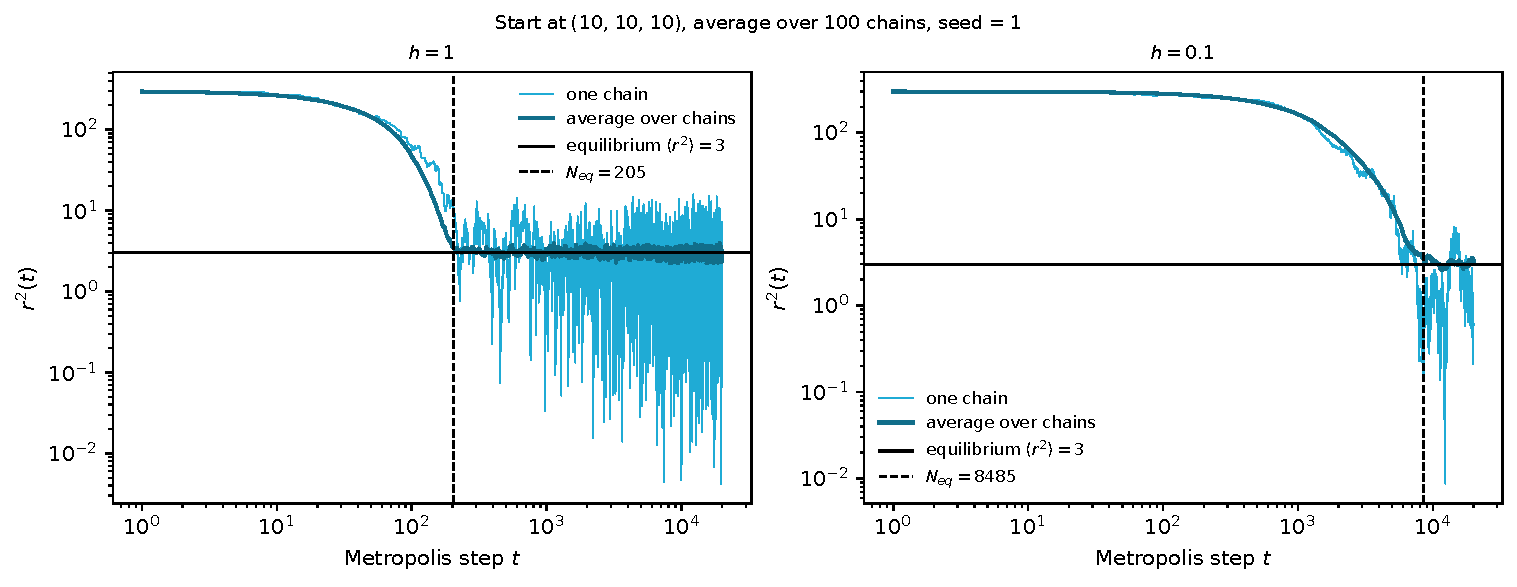
\includegraphics[width=\linewidth]{4.04-mc-integration-2-metropolis/figures/equilibration}
  \caption{Relaxation of $r^2(t)$ from $(10,10,10)$ for $h = 1$ (left) and $h = 0.1$ (right): one chain
    and the average over 100 chains of $2\times10^4$ steps. Dashed: $N_{\text{eq}}$, where the average
    first drops below $3.49$. Seed 1.}
  \label{fig:4.4-eq}
\end{figure}

\subsection{Gaussian sampling or Metropolis?}

The step size $h$ controls a trade-off (figure~\ref{fig:4.4-hscan}). For small $h$ almost every proposal
is accepted, but the steps are tiny and the chain diffuses, with $\tau_{\text{int}} \propto 1/h^2$. For
large $h$ the proposals land far in the tails and are rejected, so the chain stands still. The optimum
lies in between, $h \approx 2$--$5$ with acceptance 0.25--0.6, where $\tau_{\text{int}} \approx 5$ steps.

\begin{table}[htbp]
  \centering
  \caption{Acceptance rate and $\tau_{\text{int}}$ of $f = (x+y+z)^2$ against $h$, from $5\times10^5$
    steps per $h$ after $2\times10^4$ discarded steps, blocks of 8192 steps. Seed 1.}
  \label{tab:4.4-hscan}
  \begin{tabular}{lccccccccc}
    \toprule
    $h$ & 0.1 & 0.2 & 0.5 & 1 & 2 & 3 & 5 & 10 & 20 \\
    \midrule
    acceptance           & 0.98 & 0.96 & 0.90 & 0.81 & 0.63 & 0.48 & 0.26 & 0.053 & 0.006 \\
    $\tau_{\text{int}}$  & 1041 & 317  & 69   & 18.5 & 5.5  & 5.1  & 4.6  & 15    & 147 \\
    \bottomrule
  \end{tabular}
\end{table}

For this integral direct Gaussian sampling is clearly better. Even at the best $h$, a chain of $N$ steps
is worth only $N/(2\tau_{\text{int}}) \approx N/10$ independent points, while one Metropolis step costs
about as much as drawing three Gaussian numbers (four uniform numbers and an exponential). Gaussian
sampling is therefore at least ten times cheaper for the same error, and it needs no equilibration and no
blocking analysis. Metropolis becomes the method of choice when $w$ cannot be sampled directly, for
instance for many coupled variables as in the Ising model, or when its normalisation is unknown.

\begin{figure}[htbp]
  \centering
  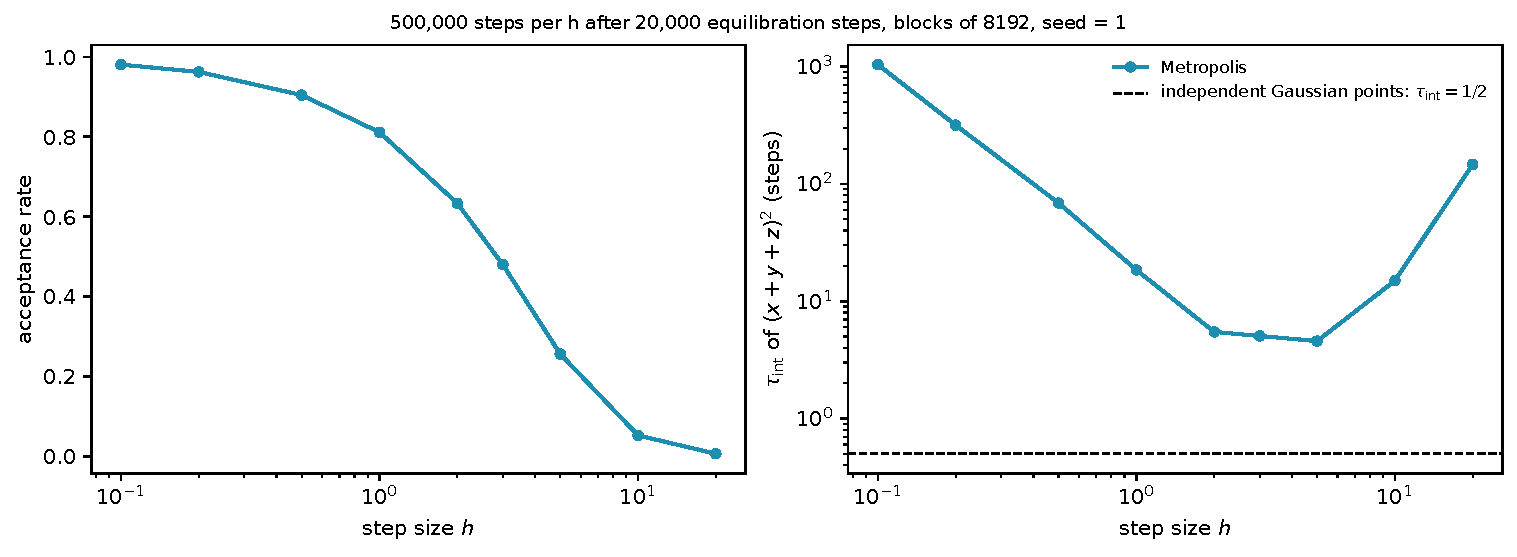
\includegraphics[width=0.85\linewidth]{4.04-mc-integration-2-metropolis/figures/h_scan}
  \caption{Step-size scan: acceptance rate (left) and integrated autocorrelation time of
    $(x+y+z)^2$ (right) against $h$, $5\times10^5$ steps per $h$ after $2\times10^4$ discarded steps,
    blocks of 8192 steps. Dashed: $\tau_{\text{int}} = 1/2$ for independent Gaussian points. Seed 1.}
  \label{fig:4.4-hscan}
\end{figure}

% Problem 4.5: Stochastic matrices
% Notes and checklist: ../Exercises/4.05-stochastic-matrices/README.md
% Figures:            \includegraphics{4.05-stochastic-matrices/figures/<name>}
\exercise{5}{Stochastic matrices}

% Suggested structure:
%   short problem description and method
%   \subsection per sub-question (analysis, simulation details, figure, discussion)
%   \kulbox[5pt]{...} with the main result, if any

% Problem 4.6: Detailed balance
% Notes and checklist: ../Exercises/4.06-detailed-balance/README.md
% Figures:            \includegraphics{4.06-detailed-balance/figures/<name>}
\exercise{6}{Detailed balance}

% Suggested structure:
%   short problem description and method
%   \subsection per sub-question (analysis, simulation details, figure, discussion)
%   \kulbox[5pt]{...} with the main result, if any

% Problem 4.7: Ising model: uniform sampling
% Notes and checklist: ../Exercises/4.07-ising-uniform-sampling/README.md
% Figures:            \includegraphics{4.07-ising-uniform-sampling/figures/<name>}
\exercise{7}{Ising model: uniform sampling}

% Suggested structure:
%   short problem description and method
%   \subsection per sub-question (analysis, simulation details, figure, discussion)
%   \kulbox[5pt]{...} with the main result, if any

% Problem 4.8: Metropolis algorithm for the Ising model
% Notes and checklist: ../Exercises/4.08-ising-metropolis/README.md
% Figures:            \includegraphics{4.08-ising-metropolis/figures/<name>}
\exercise{8}{Metropolis algorithm for the Ising model}

% Suggested structure:
%   short problem description and method
%   \subsection per sub-question (analysis, simulation details, figure, discussion)
%   \kulbox[5pt]{...} with the main result, if any

% Problem 4.9: Heat bath algorithm for the Potts model
% Notes and checklist: ../Exercises/4.09-potts-heat-bath/README.md
% Figures:            \includegraphics{4.09-potts-heat-bath/figures/<name>}
\exercise{9}{Heat bath algorithm for the Potts model}

% Suggested structure:
%   short problem description and method
%   \subsection per sub-question (analysis, simulation details, figure, discussion)
%   \kulbox[5pt]{...} with the main result, if any

% Problem 4.10: Kawasaki algorithm: the local version
% Notes and checklist: ../Exercises/4.10-kawasaki-local/README.md
% Figures:            \includegraphics{4.10-kawasaki-local/figures/<name>}
\exercise{10}{Kawasaki algorithm: the local version}

% Suggested structure:
%   short problem description and method
%   \subsection per sub-question (analysis, simulation details, figure, discussion)
%   \kulbox[5pt]{...} with the main result, if any

% Problem 4.11: Kawasaki algorithm: the non-local version
% Notes and checklist: ../Exercises/4.11-kawasaki-nonlocal/README.md
% Figures:            \includegraphics{4.11-kawasaki-nonlocal/figures/<name>}
\exercise{11}{Kawasaki algorithm: the non-local version}

% Suggested structure:
%   short problem description and method
%   \subsection per sub-question (analysis, simulation details, figure, discussion)
%   \kulbox[5pt]{...} with the main result, if any

% Problem 4.12: Hard disks
% Notes and checklist: ../Exercises/4.12-hard-disks/README.md
% Figures:            \includegraphics{4.12-hard-disks/figures/<name>}
\exercise{12}{Hard disks}

% Suggested structure:
%   short problem description and method
%   \subsection per sub-question (analysis, simulation details, figure, discussion)
%   \kulbox[5pt]{...} with the main result, if any

% Problem 4.13: Monte Carlo in continuous time for a persistent random walk
% Notes and checklist: ../Exercises/4.13-persistent-random-walk-continuous-time/README.md
% Figures:            \includegraphics{4.13-persistent-random-walk-continuous-time/figures/<name>}
\exercise{13}{Monte Carlo in continuous time for a persistent random walk}

% Suggested structure:
%   short problem description and method
%   \subsection per sub-question (analysis, simulation details, figure, discussion)
%   \kulbox[5pt]{...} with the main result, if any

% Problem 4.14: Birth-annihilation process
% Notes and checklist: ../Exercises/4.14-birth-annihilation/README.md
% Figures:            \includegraphics{4.14-birth-annihilation/figures/<name>}
\exercise{14}{Birth-annihilation process}

% Suggested structure:
%   short problem description and method
%   \subsection per sub-question (analysis, simulation details, figure, discussion)
%   \kulbox[5pt]{...} with the main result, if any

% Problem 4.15: Lotka-Volterra model
% Notes and checklist: ../Exercises/4.15-lotka-volterra/README.md
% Figures:            \includegraphics{4.15-lotka-volterra/figures/<name>}
\exercise{15}{Lotka-Volterra model}

% Suggested structure:
%   short problem description and method
%   \subsection per sub-question (analysis, simulation details, figure, discussion)
%   \kulbox[5pt]{...} with the main result, if any

% Problem 4.16: Brusselator
% Notes and checklist: ../Exercises/4.16-brusselator/README.md
% Figures:            \includegraphics{4.16-brusselator/figures/<name>}
\exercise{16}{Brusselator}

% Suggested structure:
%   short problem description and method
%   \subsection per sub-question (analysis, simulation details, figure, discussion)
%   \kulbox[5pt]{...} with the main result, if any


% ---------------------------------------------------------------
\unnumberedsection{Statement on the use of AI}
% Required by the course: state for which purposes AI was used.


% ---------------------------------------------------------------
\pagebreak
\nocite{Carlon2025}  % the lecture notes are always cited
\bibliographystyle{ieeetr}
\bibliography{References}

\end{document}
